%!TEX root = ../main.tex
\section{Introduction}
\label{sec:intro}

Machine learning (ML) has seen great success on a wide variety of applications, such as image and speech recognition, natural language processing and heath care. It has made breakthroughs due to large-scale data, high computing power, and sophisticated algorithms, but the power of humans cannot be neglected, where large-scale training data needs humans to create and some ML algorithms require humans to improve the performance iteratively. For example, ImageNet~\cite{DBLP:imagenet} is a representative benchmark that promotes the development of computer vision area. It is constructed through crowdsourcing, which is an effective way to address a wide variety of tasks by utilizing hundreds of thousands of ordinary workers (e.g., humans).
 
\begin{figure}[h!]
	\centering
	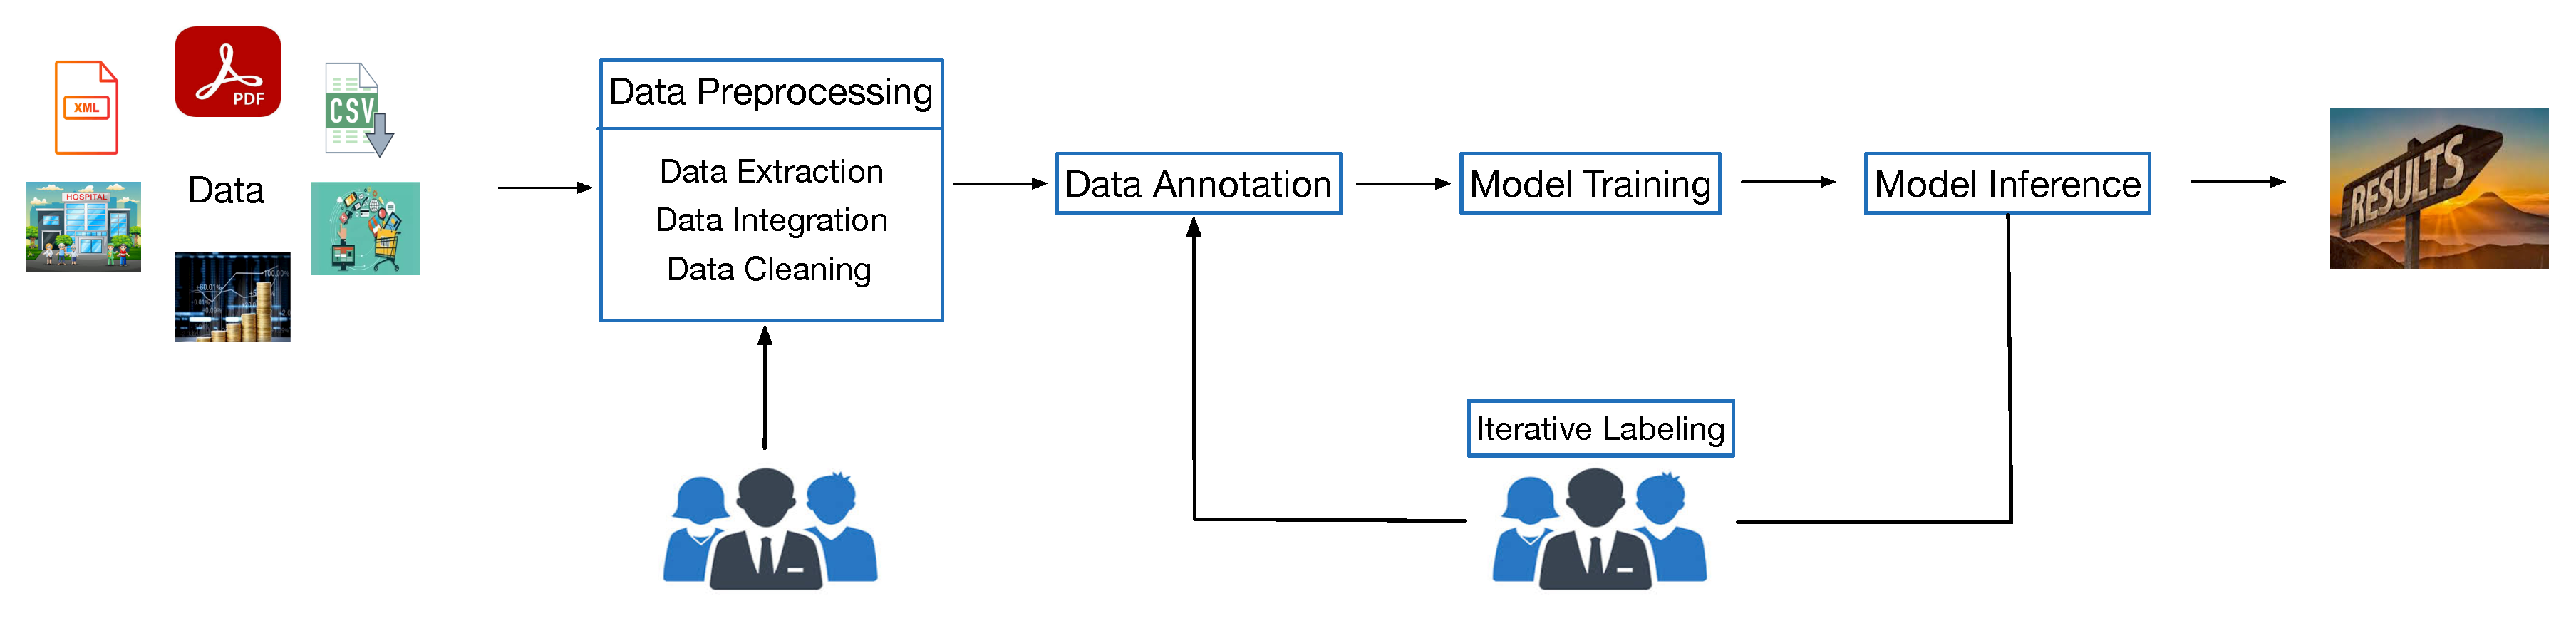
\includegraphics[scale=0.27]{submissions_new/guoliang/figs/framework.eps}
	\caption{A Human-in-the-loop Machine Learning Pipeline}
	\label{fig:framwork}
\end{figure}

Humans play important roles in the entire ML pipeline from data preparation to result inference, as shown in Figure~\ref{fig:framwork}. Before building a model, data scientists spend more than 80\% of their time in preprocessing the data~\cite{clean}, including data extraction, data integration and data cleaning. Then data is labeled and divided into training and test sets. Finally we train and test the model. Humans can contribute to all steps mentioned above.


(1) Data Extraction. In most cases,  original data we can utilize to build a model may be unstructured or semi-structured, which needs to be extracted as structured data to construct features. Data extraction is to use rules (functions) or machine learning techniques~\cite{DBLP:conf/acl/LiRC11,DBLP:conf/wsdm/NakasholeTW11, DBLP:conf/aaai/MitchellCHTBCMG15} to extract data from non-structured data, where humans can provide rules or training data. 


(2) Data Integration.  Given the structured data from multiple sources, we always have to integrate them~\cite{DBLP:journals/vldb/ChaiLLDF18,DBLP:transitivity, DBLP:crowder} to enrich the records and features. 
Data integration is used to identify duplicated records or cells in different columns that refer to the same entity, such as ``Apple iPhone 8" and``iPhone 8th", and then integrate them. 
Humans can improve the performance of data integration by providing answers of entity pairs that are hard for the computer. Also, ML techniques can also be used to address the problem, where humans can provide training data. In addition, before integrating the data, we should align the columns of different relational tables, i.e., schema matching. We can leverage human intelligence as well as knowledge bases to identify matching schemes, which are hard for the computer.

(3) Data Cleaning. In the real world, data is always dirty because of some missing values, duplicates, outliers and records that violate integrity constraints~\cite{DBLP:crowder,DBLP:conf/sigmod/ChaiC00LM20,DBLP:journals/pvldb/ChuOMIP0Y15}, so data cleaning can detect and repair these data, which are likely to  improve the ML performance. For different data cleaning tasks, we can leverage humans' cognitive ability to address them. For example, for duplicates, one can leverage machine to identify easy duplicated records and left the hard ones to humans~\cite{DBLP:crowder}. 

(4) Data Annotation and Iterative Labeling. Each record has to be labeled to construct the training set. Humans can provide high quality labels directly. Then the model is trained and tested on the labeled data. However, since humans are not free, requiring large quantities of labels is expensive. Therefore, humans will be asked to label the most interesting examples iteratively until a good performance is achieved.

(5) Model training and inference.  For different machine learning tasks, like classification and clustering, there are different techniques that leverage humans' labels to train and infer the results. For classification, one can utilize techniques like deep learning,  expectation maximization or graph model to deduce the results based on noisy human labeled data. For clustering,   a straightforward method is to leverage a human-machine hybrid method to cluster these examples(e.g. video or images) that are hard to cluster purely by computers. In addition, generative models can also be applied to cluster examples according to multiple criteria.

Although  humans contribute to different modules in the ML pipeline, there are several common important problems in human-in-the-loop machine learning. The first is quality improvement, Humans are likely to make mistakes no matter what kinds of tasks they do because they may have different levels of expertise, and an untrained human is not qualified to accomplish certain tasks. To achieve high quality labels, we need to tolerate human errors and infer high quality results from noisy answers. Secondly, Since humans are not free, if there are large numbers of tasks, it is expensive to leverage humans to address all of them. Therefore, several techniques are proposed such as pruning, answer deduction and sampling. Thirdly, generally speaking, humans are much slower than the computer. To accomplish the tasks efficiently, we should reduce the latency, which is the time from the user submits the first task to the final answer is returned.  Fourthly, given a task, a user does not always have enough budget to label a large number of training data. Therefore, 
active learning is proposed to  involve humans to label the most interesting examples iteratively so that the examples in each iteration affect the model as much as possible.  Lastly, in active learning, we assume the labels provided by humans are perfect, but it does not hold in reality. Therefore, weak supervision is proposed to obtain a relative high quality result through a large number of weak labels, which are provided by humans with different qualities or functions (rules).


\iffalse
(1) Quality improvement. Humans are likely to make mistakes no matter what kinds of tasks they do because they may have different levels of expertise, and an untrained human is not qualified to accomplish certain tasks. To achieve high quality labels, we need to tolerate human errors and infer high quality results from noisy answers. Therefore, we should model the humans' quality and tasks' difficulty, assign  tasks to appropriate humans and infer final results. We discuss quality improvement methods in Section ~\ref{subsec:quality}.


(2) Cost reduction.  Since humans are not free, if there are large quantities of tasks, it is expensive to leverage humans to address all of them. For example, in entity resolution, if there are 10, 000 records, there will be about 50 million pairs. Even if the price per pair is 1 cent, it still takes much money. There are several effective cost reduction techniques. The first is pruning, which utilizes machine-based algorithms to remove some unnecessary(easy) tasks. The second is task selection, which prioritizes which tasks will be assigned to humans. The third is the answer deduction, which utilizes current answers to deduce the results of other tasks.
The fourth is sampling, which samples a subset of tasks to ask humans and then propagates the answers to the entire dataset.  We review cost reduction methods in Section~\ref{subsec:cost}.


(3) Latency reduction. Generally speaking, humans are much slower than the computer. To accomplish the tasks efficiently, we should reduce the latency, which is the time from the user submits the first task to the final answer is returned.  There are mainly two strategies for latency control.  The first is the round-based model, which leverages the idea that tasks can be published in multiple rounds. If there are enough humans to answer them, the latency of answering tasks in each round can be regarded as constant time. Thus the overall latency is modeled as the number of rounds. The second one is the statistical model, which uses  the collected statistics from previous  tasks to build statistical models that can estimate  the humans’ latency for different tasks. We review latency control methods in Section ~\ref{subsec:latency}.


(4) Active learning.  Given a task, a user does not always have enough budget to label a large number of training data. Therefore, 
active learning is proposed to  involve humans to label the most interesting examples iteratively so that the examples each iteration impact the model as much as possible. There are several methods to describe how interesting each example is, including uncertainty, expected model change, expected error reduction, etc.   We review latency control methods in Section ~\ref{subsec:active_learning}.
 %It always assumes that humans can provide accurate answers. The key challenge is that given a limited budget, how to select the most appropriate  examples in each iteration. Active learning has been covered extensively in  surveys ~\cite{settles2009active, DBLP:reference/sp/2015rsh}, so we only cover the most prominent techniques in this part. Next, we will introduce several strategies of selecting items to be labeled in each iteration.


(5) Weak supervision. In active learning, we always assume the labels provided by humans are perfect, but it does not hold in reality. Therefore, weak supervision is proposed to obtain a relative high quality result through weak labels, which are provided by humans with different qualities or functions(rules).  Weak supervision can be categorized into two classes. The first one is data programming that generates a large number of weak labels using multiple labeling functions, which are written bu humans. The second one is fact extraction, which generates weak labels using existing sources like knowledge bases. We review weak supervision  in Section ~\ref{subsec:weak}.

\fi

In a word, we will introduce what humans can contribute in the machine learning pipeline in Section~\ref{sec:pipeline}. Next, several significant human-in-the-loop techniques are introduced in Section~\ref{sec:overview}. Then we discuss some open challenges and opportunities in Section~\ref{sec:future} and conclude in Section ~\ref{sec:con}.

%Given the above general techniques about human-based machine learning, we introduce how to apply them in different modules in ML pipeline in section ~\ref{sec:pipeline}, including data extraction, data integration, data cleaning  and iterate labeling. Then we discuss some open challenges and opportunities in section ~\ref{sec:future} and conclude in section ~\ref{sec:con}.